\section{Theorie}
\subsection{Strömende Flüssigkeiten und Gase}



\subsubsection{Grundbetrachtungen}
Strömende Flüssigkeiten und Gase unterscheiden sich hauptsächlich in zwei Punkten. Zum einen sind die Dichten von Flüssigkeiten um etwa drei Größenordnungen größer als bei Gasen. Zum anderen sind Flüssigkeiten in guter Näherung inkompressibel, was auf Gase nicht zutrifft.

Um die makroskopische Bewegung von Flüssigkeiten und Gasen beschreiben zu können, ist es nötig alle Kräfte zu kennen, die auf ein Volumenelement $ \Delta V $ wirken. Als Kräfte kommen dabei Kräfte durch Druckdifferenzen $ \vec{F}_p $, die Schwerkraft $ \vec{F}_g $ und Reibungskräfte $ \vec{F}_R $ zwischen Schichten des strömenden Mediums in Frage. Hier bezeichnet $p$ den Druck und $\rho$ die Dichte. Dabei gilt:

\begin{equation}
\vec{F}_p = -{\bf grad}(p) \cdot \Delta V
\end{equation}
\begin{equation}
\vec{F}_g = \rho \cdot \vec{g} \cdot \Delta V
\end{equation}
Die Reibungskraft $ \vec{F}_R $ wird weiter unten noch behandelt.

Mit $ \vec{F} := \vec{F}_p + \vec{F}_g + \vec{F}_R $ ergibt sich für die Newtonschen Bewegungsgleichungen:

\begin{equation}
\vec{F} = \Delta m \ddot{\vec{r}} = \rho \cdot \Delta V \cdot \frac{d \vec{u}}{dt}
\label{form:Newton}
\end{equation}
Dabei ist $ \vec{u} = \frac{d \vec{r}}{dt} $ die Strömungsgeschwindigkeit des Volumenelements $ \Delta V $.\\
\\Kennt man die Strömungsgeschwindigkeit $ \vec{u} ( \vec{r} , t) $ an allen Orten $ \vec{r} $ und zu jedem Zeitpunkt $ t $, so kennt man die makroskopische Bewegung der gesamten Flüssigkeit.

Eine Strömung heißt stationär, wenn $ \vec{u} ( \vec{r} , t) \equiv \vec{u} ( \vec{r} ) $ nicht von $t$ abhängt.
Flüssigkeiten, bei denen $ \Vert \vec{F}_R \Vert \ll \Vert \vec{F}_p \Vert + \Vert \vec{F}_g \Vert $, bezeichnet man als ideale Flüssigkeiten, während Flüssigkeiten, bei denen $ \Vert \vec{F}_R \Vert \gg \Vert \vec{F}_p \Vert + \Vert \vec{F}_g \Vert $, als viskos oder zäh bezeichnet werden.

Die Kurve $ \vec{r} (t) $ eines Flüssigkeitselements $ \Delta V $ nennt man Stromlinie. (Abb. \ref{fig:8-1}) Strömungen heißen laminar, wenn sich die Stromlinien nebeneinander bewegen und sich nicht vermischen. (Abb. \ref{fig:8-5}) Laminare Strömungen liegen immer dann vor, wenn die inneren Reibungskräfte im Vergleich zu den anderen Kräften groß sind. Sind die inneren Reibungskräfte allerdings klein im Vergleich zu Kräften, wie z.B. solche die an Hindernissen auftreten, bilden sich Wirbel. Solche Strömungen bezeichnet man als turbulent. (Abb. \ref{fig:8-6})

\begin{figure}
        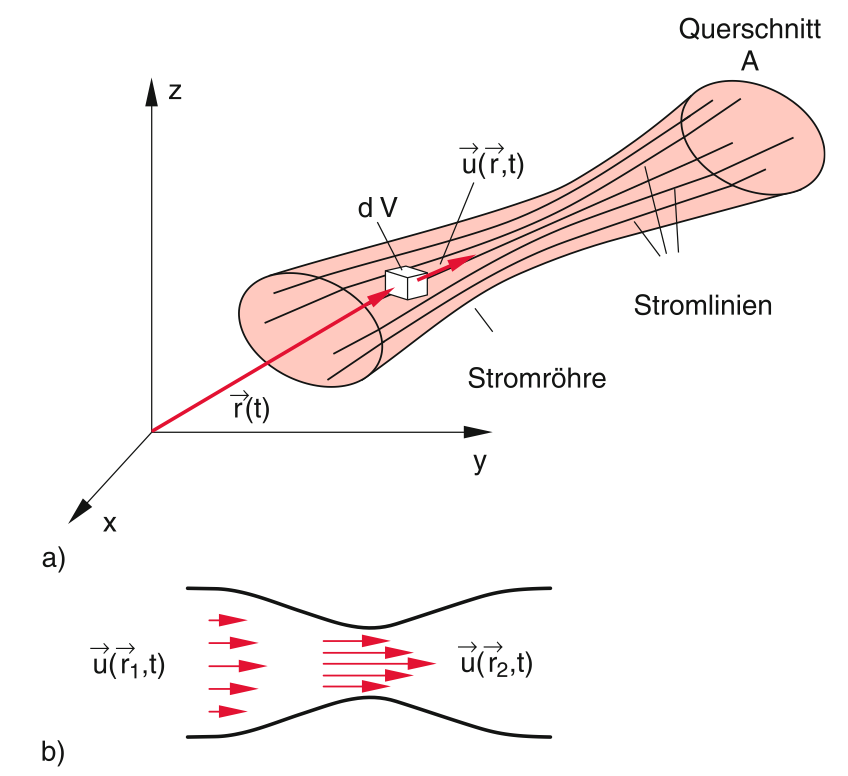
\includegraphics[width=.9\textwidth]{images/8-1}
\caption{(a) Stromlinien und Strömungsgeschwindigkeit $ \vec{u}(\vec{r},t) $ ; (b) Strömungsfeld zu einem bestimmten Zeitpunkt $t$ }
\label{fig:8-1}
\end{figure}

\begin{figure}
		\centering
        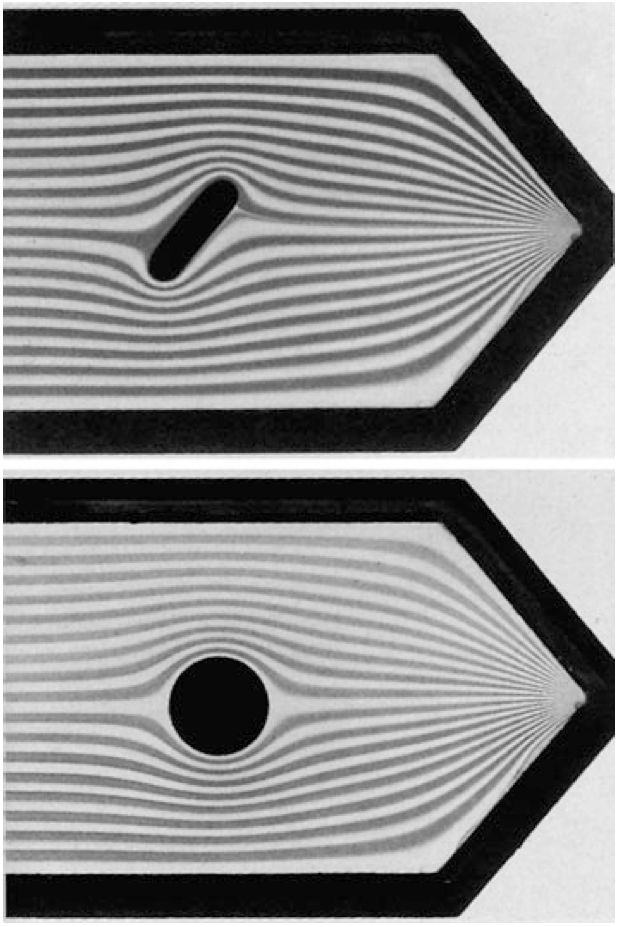
\includegraphics[width=.9\textwidth]{images/8-5}
\caption{Beispiele laminarer Strömungen}
\label{fig:8-5}
\end{figure}

\begin{figure}
	\centering
        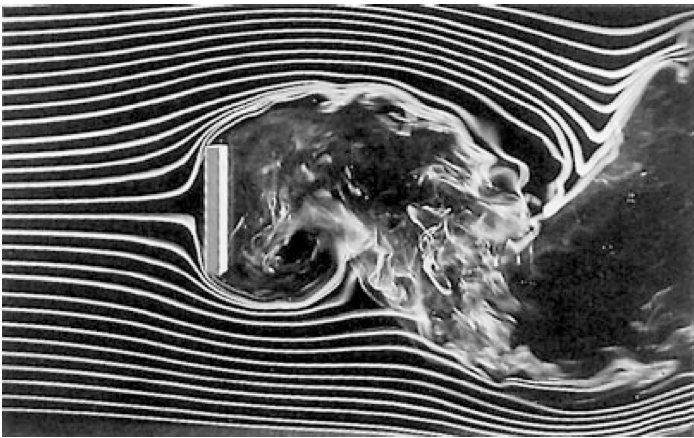
\includegraphics[width=.9\textwidth]{images/8-6}
\caption{Beispiel einer turbulenten Strömung}
\label{fig:8-6}
\end{figure}

\subsubsection{Die Kontinuitätsgleichung}
Sei $ V $ ein beliebiges Volumen. $V$ enthält zur Zeit $t$ die Masse:

\begin{equation}
M(t) = \iiint_V \rho (t) dV
\end{equation}
Aufgrund der Massenerhaltung kann sich die Masse in $V$ nur dann ändern, wenn Masse durch die Oberfläche $ \partial V $ ein- oder ausströmt. Sei $ \vec{j} = \rho \cdot \vec{u} $ die Massenstromdichte. Dann gilt wegen der Massenerhaltung:

\begin{equation}
-\frac{\partial M}{\partial t} = \iint_{\partial V} \vec{j} \cdot d \vec{\sigma} = \iint_{\partial V} \rho \cdot \vec{u} \cdot d \vec{\sigma}
\end{equation}
Dabei ist $ d \vec{\sigma} $ der Flächennormalenvektor. Also folgt mit dem Satz von Gauß:

\begin{equation}
-\frac{\partial M}{\partial t} = -\frac{\partial}{\partial t} \iiint_V \rho dV = \iiint_V (-\frac{\partial}{\partial t} \rho) dV = \iiint_V {\bf div}(\rho \cdot \vec{u})dV = \iint_{\partial V} \rho \cdot \vec{u} \cdot d \vec{\sigma}
\label{form:viele Integrale}
\end{equation}
Da Gleichung (\ref{form:viele Integrale}) für beliebige $V$ gilt, folgt:

\begin{equation}
\boxed{\frac{\partial \rho}{\partial t} + {\bf div}(\rho \cdot \vec{u}) = 0}
\label{form:Kontinuitätsgl.}
\end{equation}
Diese Gleichung nennt man die Kontinuitätsgleichung. Sie drückt aus, dass Masse erhalten ist. Im Fall von inkompressiblen Flüssigkeiten gilt: $ \rho = const. $ . Deshalb vereinfacht sich Gleichung (\ref{form:Kontinuitätsgl.}) zu:

\begin{equation}
{\bf div}(\vec{u}) = 0
\end{equation}

\subsubsection{Die Euler-Gleichung}
Für $ \frac{d \vec{u}}{dt} $ gilt:

\begin{equation}
\frac{d \vec{u}}{dt} = \frac{\partial \vec{u}}{\partial t} + \frac{\partial \vec{u}}{\partial x} \frac{\partial x}{\partial t} + \frac{\partial \vec{u}}{\partial y} \frac{\partial y}{\partial t} + \frac{\partial \vec{u}}{\partial z} \frac{\partial z}{\partial t} = \frac{\partial \vec{u}}{\partial t} + \frac{\partial \vec{u}}{\partial x} u_x + \frac{\partial \vec{u}}{\partial y} u_y + \frac{\partial \vec{u}}{\partial z} u_z = \frac{\partial \vec{u}}{\partial t} + (\vec{u} \cdot \nabla) \vec{u}
\label{form:herleitung euler}
\end{equation}
Aufgrund der Gleichungen (\ref{form:Newton}) und (\ref{form:herleitung euler}) ergibt sich für die Bewegungsgleichung einer idealen Flüssigkeit:

\begin{equation}
\boxed{\frac{d \vec{u}}{dt} = \frac{\partial \vec{u}}{\partial t} + (\vec{u} \cdot \nabla) \vec{u} = \vec{g} - \frac{1}{\rho} {\bf grad} (p)}
\end{equation}
Diese Gleichung nennt man die Euler-Gleichung. Sie bildet die Grundlage der Hydrodynamik idealer Flüssigkeiten.

\subsubsection{Die Bernoulli-Gleichung}
Hier wird ein Fluid (Flüssigkeit oder Gas) betrachtet, das horizontal durch ein Rohr mit veränderlichem Querschnitt fließt. (Abb. \ref{fig:8-8}) Die Bernoulli-Gleichung folgt dann aus der Energieerhaltung. Strömt ein Fluid durch ein Rohr, dessen Querschnitt variabel ist, so muss das Fluid aufgrund der Kontinuitätsgleichung \ref{form:Kontinuitätsgl.} an Stellen mit kleinerem Querschnitt schneller fließen. Ein Volumen $ \Delta V_1 = A_1 \cdot \Delta x_1 $ hat dort also eine größere kinetische Energie.

\begin{figure}
		\centering
        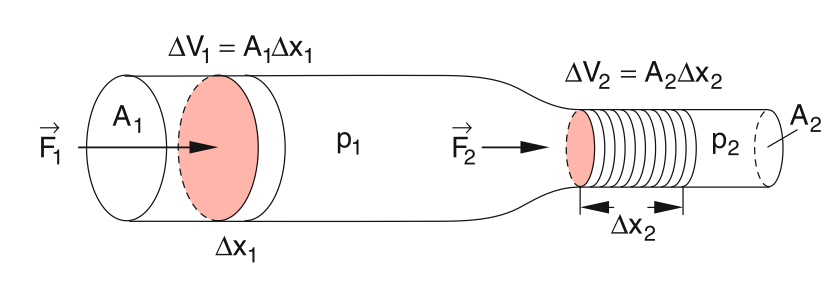
\includegraphics[width=.9\textwidth]{images/8-8}
\caption{ Rohr mit variablem Querschnitt zur Herleitung der Bernoulli-Gleichung }
\label{fig:8-8}
\end{figure}

Um das Volumen $ \Delta V_1 $ um $ \Delta x_1 $ gegen $ p_1 $ zu verschieben, ist eine Arbeit $ \Delta W_1 $ nötig. Analoges gilt für $ \Delta V_2 $. Es gilt dann:

\begin{equation}
\Delta W_1 = F_1 \cdot \Delta x_1 = p_1 \cdot A_1 \cdot \Delta x_1 = p_1 \cdot \Delta V_1
\end{equation}
\begin{equation}
\Delta W_2 = F_2 \cdot \Delta x_2 = p_2 \cdot A_2 \cdot \Delta x_2 = p_2 \cdot \Delta V_2
\end{equation}
Die kinetische Energie des Volumenelements $ \Delta V $ ist $ E_{kin} = \frac{1}{2} \Delta m u^2 = \frac{1}{2} \rho u^2 \Delta V $. Für ideale Flüssigkeiten muss nun die Summe aus kinetischer und potentieller Energie konstant sein. Deshalb folgt:

\begin{equation}
p_1 \Delta V_1 + \frac{1}{2} \rho u_1^2 \Delta V_1 = p_2 \Delta V_2 + \frac{1}{2} \rho u_2^2 \Delta V_2
\end{equation}
Für inkompressible Flüssigkeiten gilt nun $ \Delta V_1 = \Delta V = \Delta V_2 $. Damit ergibt sich:

\begin{equation}
p_1 + \frac{1}{2} \rho u_1^2 = p_2 + \frac{1}{2} \rho u_2^2
\label{form:Pre-Bernoulli}
\end{equation}
Da Gleichung (\ref{form:Pre-Bernoulli}) für beliebige Querschnitte gilt, folgt die Bernoulli-Gleichung:

\begin{equation}
\boxed{p + \frac{1}{2} \rho u^2 = p_0 = const.}
\label{form:Bernoulli-Gleichung}
\end{equation}
$ p_0 $ heißt Gesamtdruck, $ p_S = \frac{1}{2} \rho u^2 $ heißt Staudruck und $p$ ist der statische Druck der strömenden Flüssigkeit.

Verläuft die Strömung durch schräge Rohre (Abb. \ref{fig:8-11}), ergibt sich die allgemeinere Gleichung:

\begin{equation}
p + \rho g z(x) + \frac{1}{2} \rho u^2(x) = p_0 = const.
\end{equation}
Dabei ist $z(x)$ die Höhe am Ort $x$.

\begin{figure}
	\centering
        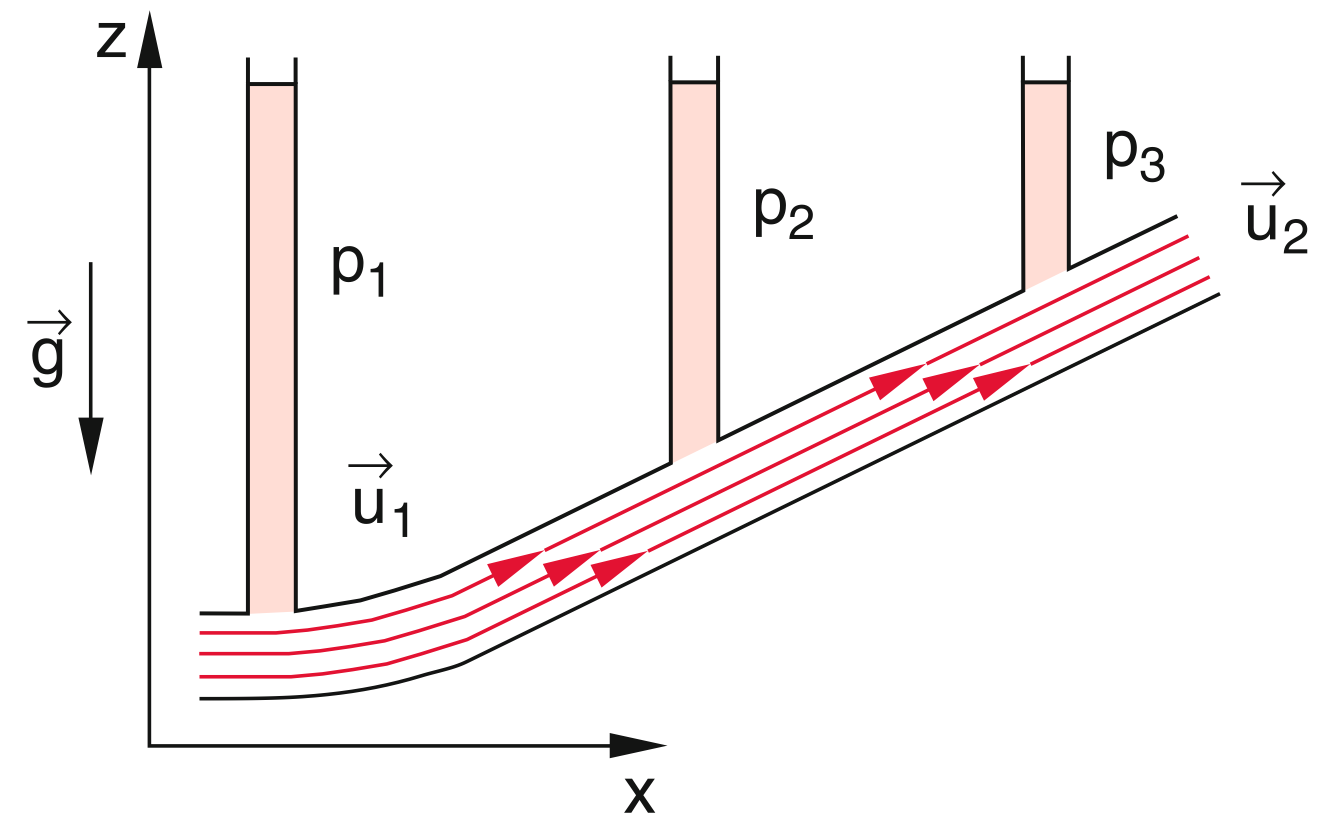
\includegraphics[width=.9\textwidth]{images/8-11}
\caption{ Strömung durch ein schräges Rohr }
\label{fig:8-11}
\end{figure}

\subsubsection{Die Navier-Stokes-Gleichung}
Die Bewegungsgleichung für reale viskose strömende Fluide kann angegeben werden, wenn auch $ \vec{F}_R $ genauer bestimmt ist. Für viskose Fluide gilt:

\begin{equation}
\vec{F}_R = \eta {\bf \Delta} \vec{u} \Delta V
\end{equation}
Dabei ist $ {\bf \Delta} = \nabla \cdot \nabla = \frac{\partial^2}{\partial x^2} + \frac{\partial^2}{\partial y^2} + \frac{\partial^2}{\partial z^2} $ der Laplace-Operator. Aus \ref{form:Newton} folgt nun mit Hilfe von Gleichung (\ref{form:herleitung euler}) die Navier-Stokes-Gleichung:

\begin{equation}
\boxed{\rho (\frac{\partial}{\partial t} + \vec{u} \cdot \nabla ) \vec{u} = - {\bf grad}(p) + \rho \cdot \vec{g} + \eta {\bf \Delta} \vec{u}}
\end{equation}
Die Lösung der Navier-Stokes-Gleichung ist laut dem Clay Mathematics Institute sogar Teil der Millenium-Probleme. Deshalb werden wir uns hier nicht weiter mit der Navier-Stokes-Gleichung befassen. \footnote{nach \cite[212ff.]{troeder}}

\subsection{Strömungsmesstechnik}
\subsubsection{Grundsätzliche Betrachtungen}
Betrachtet man ein Fluid, ist ihm zunächst nicht anzusehen, ob es strömt oder nicht. Dies wird erst durch Fremdkörper wie z.B. Rauch, Farbstoff, Strömungsfäden oder anderes ermöglicht. Es wird also in der Praxis unmöglich sein tatsächlich $ \vec{u} ( \vec{r} , t) $ für alle $ \vec{r} $ und $t$ zu messen. Deshalb ist man auf indirekte Methoden wie z.B. die  Messung von Druckdifferenzen oder die Messung der Kraft auf einen in der Strömung befindlichen Körper angewiesen. Außerdem sind Messinstrumente oft nur dazu in der Lage den Betrag oder die Richtung von $ \vec{u} $ zu bestimmen. Dabei ist außerdem zu beachten, dass Instrumente zur Messung des Betrags von $ \vec{u} $ oft eine Richtungsempfindlichkeit besitzen, sodass vor der Messung des Betrags die Kenntnis der Richtung von $ \vec{u} $ erforderlich ist.

Die Grundlage zur Bestimmung von Strömungsgeschwindigkeiten durch Druckmessung bildet die Bernoulli-Gleichung \ref{form:Bernoulli-Gleichung}. Stellt man diese nach $u$ um, ergibt sich eine Formel zur Bestimmung der Strömungsgeschwindigkeit des Fluids:

\begin{equation}
\boxed{u = \sqrt{\frac{2}{\rho} (p_0 - p)} = \sqrt{\frac{2}{\rho} p_d}}
\label{eq:Geschwindigkeitsformel}
\end{equation} 
Dabei ist $ p_d := p_0 - p $ der dynamische Druck. In der Praxis wird deshalb oft eine Messung des Gesamtdrucks und des statischen Drucks durchgeführt, um aus der Differenz auf die Geschwindigkeit des strömenden Fluids schließen zu können.

\subsubsection{Sonden zur Messung des Gesamtdrucks (Pitotrohre)}
Im vorderen Teil eines Körpers stellt sich der Gesamtdruck ein, der dort durch Anbringen einer Bohrung gemessen werden kann. Mit einem parallel zur Strömung ausgerichteten Rohr hat schon Henri Pitot (1732) als erster Strömungsgeschwindigkeiten gemessen. Deshalb bezeichnet man Gesamtdruckrohre als Pitotrohre. Um die Richtungsempfindlichkeit von Pitotrohren zu verbessern wurden verschiedene Kopfformen entwickelt, unter anderem auch ein umhülltes Pitotrohr (siehe rechts unten \aref{sonden}). Der maximale Winkelbereich, um unter $ 1 \% $ Fehler zu bleiben, hängt stark von der jeweiligen Bauweise ab. Er kann bei einer scharfen Vorderkante $ \pm 10^{\circ} $ betragen und reicht beim umhüllten Pitotrohr bis zu $ \pm 60^{\circ} $. Diese Werte sind jedoch nur Richtwerte. Weiterhin hängt die Richtungsempfindlichkeit auch noch von der Mach-Zahl (Verhältnis von Strömungsgeschwindigkeit zu Schallgeschwindigkeit) ab, mit höherer Geschwindigkeit wird auch die Richtungsempfindlichkeit größer.
%Abb. zu versch. Köpfen
\begin{figure}
	\centering
	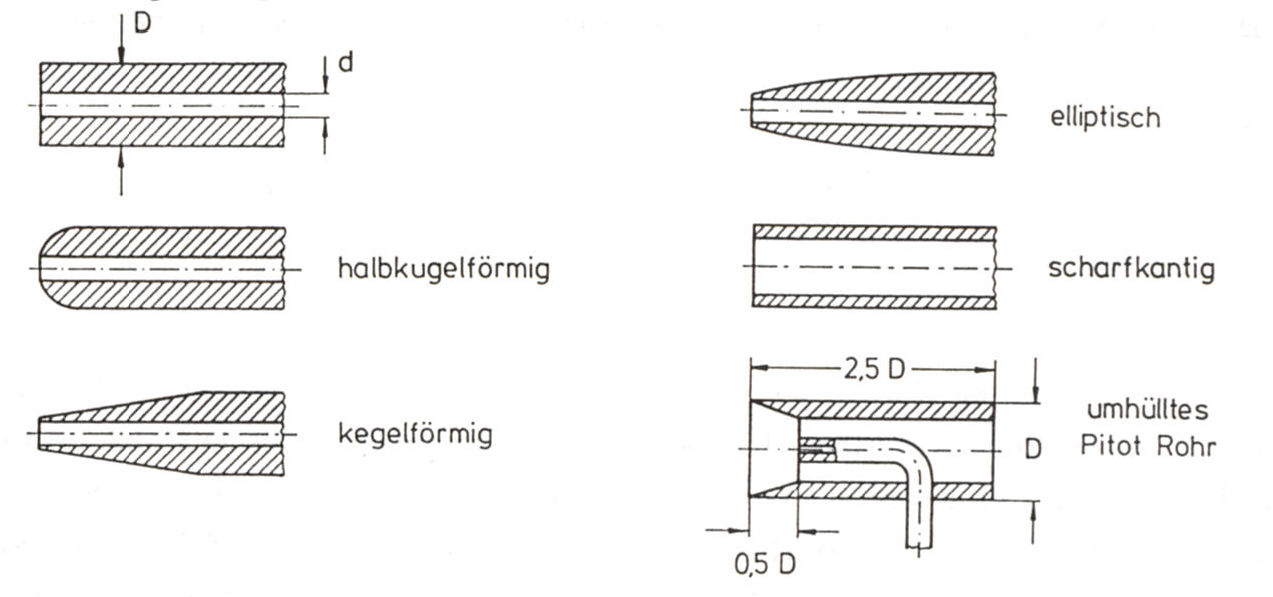
\includegraphics[width=\textwidth]{images/sonden.jpg}
	\caption{Verschiedene Ausführungen der Sondenköpfe}
	\label{sonden}
\end{figure}

\subsubsection{Sonden zur Messung des statischen Drucks}
Zur Messung des statischen Drucks (siehe \aref{statisch}) wird ein vorne geschlossenes Rohr mit seitlichen Bohrungen verwendet. Die Bohrungen dürfen dabei keinen Grat oder ähnliches aufweisen, da sonst die Messergebnisse verfälscht werden. Außerdem muss die Bohrung exakt senkrecht zur Wand und damit auch zur Strömung sein.
%Abb. einfügen
\begin{figure}
	\centering
	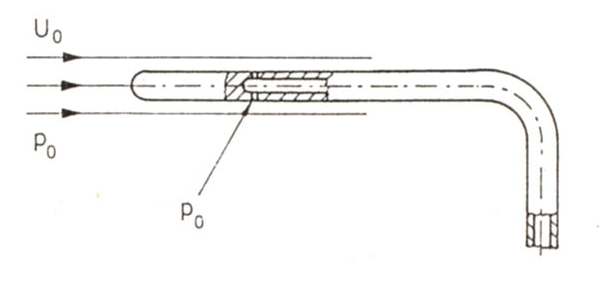
\includegraphics[width=0.8\textwidth]{images/statisch}
	\caption{Sonde zur Messung des statischen Drucks}
	\label{statisch}
\end{figure}

\subsubsection{Sonden zur gleichzeitigen Messung des Gesamtdrucks und des statischen Drucks (Prandtlsonden)}
Eine Prandtlsonde (siehe \aref{prandtl}) ist Pitotrohr und statische Drucksonde in einem und kann daher direkt zur Messung des dynamischen Drucks verwendet werden. Bei der Prandtlsonde ist die Messung des statischen Drucks problematisch, da es wichtig ist, dass sich die Bohrungen hierfür nicht zu weit vorne, aber auch nicht zu weit hinten befindet. Beides führt zu Fehlern bei der Messung des statischen Drucks. Werden diese Bohrungen jedoch korrekt platziert, gleichen sich die Messfehler gerade gegenseitig aus. Hier soll jedoch nicht weiter auf diesen Aspekt eingegangen werden, da bei unseren Messungen ein Pitotrohr verwendet wurde.  \footnote{nach \cite{elmann}}



%Abb. einfügen
\begin{figure}
	\centering
	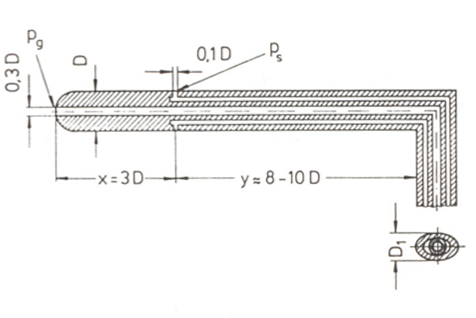
\includegraphics[width=0.7\textwidth]{images/prandtl}
	\caption{Prandtlsonde}
	\label{prandtl}
\end{figure}
